\documentclass[10pt,a4paper]{article}
\usepackage[margin=2cm]{geometry}
\usepackage{graphicx}
\usepackage{amsmath,amssymb}
\usepackage{array}
\usepackage{amsthm}
\usepackage[section]{placeins}
\usepackage{setspace}
\usepackage{enumerate}
\usepackage{fullpage}
%\usepackage{subfigure}
\usepackage{caption}
\usepackage{subfiles}
% \usepackage{subcaption}
\usepackage{tikz}
\usepackage{algorithm}
\usepackage{algorithmic}
\usepackage{listings}
\usepackage{color}
\usepackage[caption=false]{subfig}
\usepackage{xcolor, colortbl}


% \definecolor{green}{rgb}{0.1,0.1,0.1}

\parindent 0pt
\everymath{\displaystyle}
\title{CSA 250 : Deep Learning Project II \\ Report}
\author{Magare Aadesh Gajanan (15605)}
\date{\today}

\setlength{\parskip}{0.5em}

\newtheorem{theorem}{Theorem}
\newtheorem{definition}{Definition}
\newtheorem{proposition}{Proposition}
\newtheorem{corollary}{Corollary}
\newtheorem{lemma}{Lemma}

\DeclareMathOperator*{\argmin}{arg\,min}
\DeclareMathOperator{\scriptL}{\mathcal{L}}
\newcommand{\olambda}{\overline{\lambda}}


\begin{document}

\maketitle
\section{Task}

This project is to implement neural network and convolutional neural network for the task of image classification. We need to train the classifiers using Fashion-MNIST clothing images.

\section{Dataset}

For training and testing of our classifiers, we will use the Fashion-MNIST dataset. The Fashion-MNIST is a dataset of Zalando's article images, consisting of a training set of 60,000 examples and a test set of 10,000 examples. Each example is a 28x28 grayscale image, associated with a label from 10 classes.

	The training set is further divided into training and validation set splitting the data into 85\% and 15\% parts. This reduced training set is used to train both the architectures while validation set is used for hyper-parameter tuning. Finally tuned model is evaluated on the test dataset and final results are reported.
	
\section{Approach}
I tried two different architectures for the task i.e. Feed Forward neural network and Convolutional neural network. For both the approaches I'll present how I arrived on final architecture, justify different architectural choices and tune hyper parameters.

\subsection{Feed Forward Neural Network (Multi-Layer Perceptron)}

Each training example is a 28x28 grayscale image i.e. 784 pixels when flattened. Thus starting with simple model with 2 hidden layers with 256 and 64 hidden units respectively. Since output is one of the 10 classes, throughout experiments output layer would have 10 units. It's a multi-class classification problem thus I'll be using CrossEntropy loss. ReLu is good default choice for activation function to begin experiment, we'll see how other activation functions compare. I have used Adam optimizer with 1e-3 learning rate, which will be tuned during hyper parameter tuning phase.

	This simple baseline model gives accuracy of 90.21\% on the validation set. Figure \ref{mlploss} shows the training loss decreasing with no of epocs. Training is stopped at 30 epocs since further training gives no performance gain in validation set accuracy. We'll stick to 30 epocs for further experiments for fair comparison. \\

\begin{figure}[h!]
\begin{center}
	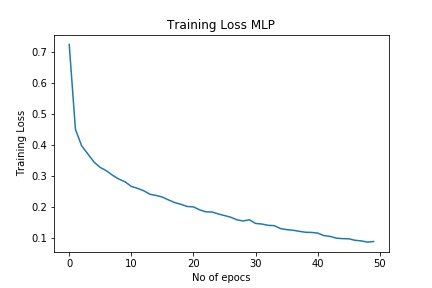
\includegraphics[width=0.85\linewidth]{training_mlp.jpg}
	\caption{MLP Loss}
	\label{mlploss}
\end{center}
\end{figure}

\pagebreak

	Next we'll increase the capacity of network by adding additional layers. Figure \ref{mlpval} shows the performance of the network with additional layers. Slight drop in accuracy suggest the possibility of over-fitting in network. We'll keep the no of hidden layers to 3 where the over-fitting has just started and explore regularization methods to further increase accuracy.

\begin{figure}[h!]
\begin{center}
	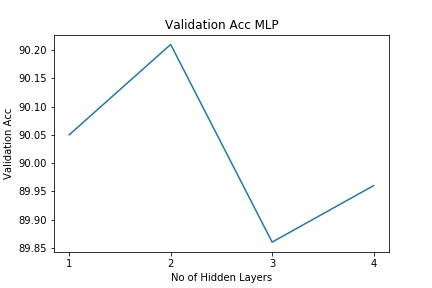
\includegraphics[width=0.85\linewidth]{val_mlp.jpg}
	\caption{MLP Val Acc}
	\label{mlpval}
\end{center}
\end{figure}
	
\textbf{Regularization:} Following forms of regularization were tried, it was also observed that combining multiple forms of regularization does not give good performance.\\

\begin{enumerate}
\item \textbf{Normalization} We'll use normalize transform on the dataset to get 0 mean and unit variance. Additionally we'll apply \textbf{BatchNorm} after every hidden layer. BatchNorm has been shown to be very useful in CNNs however here we didn't see performance gain due to it. Resultant model gives 89.40\% validation accuracy. 

\item \textbf{L2 penalty} L2 regularization is another widely used regularization method for linear models. It's rarely used in DNN computer vision tasks, here the resultant model gives 83.65\% accuracy.

\item \textbf{Dropout} It's the de-facto regularization method for computer vision tasks and shown to prevent over-fitting in wide variety of network architectures. Here the resultant model gives 90.27\% accuracy.

\item \textbf{Data Augmentation} It is often used when dealing with smaller datasets where we augment the dataset to increase the size, it helps in reducing over-fitting. We'll use RandomHorizontalFlip for data augmentation. Here the resultant model gives 89.76\% accuracy. Adding random noise for data augmentation shows no improvement but further reduces accuracy.

\end{enumerate}

Next we try different activation functions i.e. Sigmoid, Tanh, ReLU. as expected ReLU performs the best from the alternatives. Sigmoid and Tanh gives 0.36\% and 0.65\% reduction in accuracy respectively when compared against ReLU.

\textbf{Hyper-Parameters tuning} After choosing the best model so far i.e. model with 3 hidden layers and dropout regularization with ReLU activation function, we'll tune the remaining hyper-parameters.
\begin{enumerate}
\item \textbf{Learning rate} is probably the most important hyper parameter, I've started with good default of 1e-3 and used "ReduceLROnPlateau" learning rate scheduler in PyTorch. It gradually decreases the learning rate upon reaching a plateau. Here for the scheduler to work better, the model is trained for 50 epocs.
\item \textbf{Batch Size} affects both the training speed and the accuracy of resultant model, I have tried several values for batch size and 512 gives the best results.

\end{enumerate}

After all hyper-parameter tuning and using learning rate scheduler (training upto 60 epocs) we get a validation accuracy of \textbf{91.22\%.}. Table \ref{table:1} gives the summary of overall experiments.

\begin{table}[h!]
\centering
\begin{tabular}{|c| c|} 
 \hline
 Model & Validation Accuracy (\%) \\
 \hline\hline
 Baseline (2 hidden layers) & 90.21 \\ 
 \hline
 3 hidden layers with BatchNorm & 89.40 \\ 
 \hline
 3 hidden layers with L2 penalty & 83.65 \\ 
 \hline
 3 hidden layers with dropout & 90.27 \\ 
 \hline
 3 hidden layers with data aug & 89.76 \\ 
 \hline
 3 hidden layers tuned hyper params & \textbf{91.22} \\ 
 \hline
\end{tabular}
\caption{Summary of different architectural choices (MLP) }
\label{table:1}
\end{table}

Finally we take the best performing model and test the performance on actual test set. Here it gives \textbf{accuracy of 90.34\%}. Figure \ref{mlpcm} shows the confusion matrix for test data. As expected most of confusion lies between classes such as Shirt vs Tshirt, Coat vs Pullover and Shirt vs Pullover which is justified given the visual similarity between the classes. This suggests that model has captured the differences between classes to a good extent.

\begin{figure}[h!]
%\begin{center}
	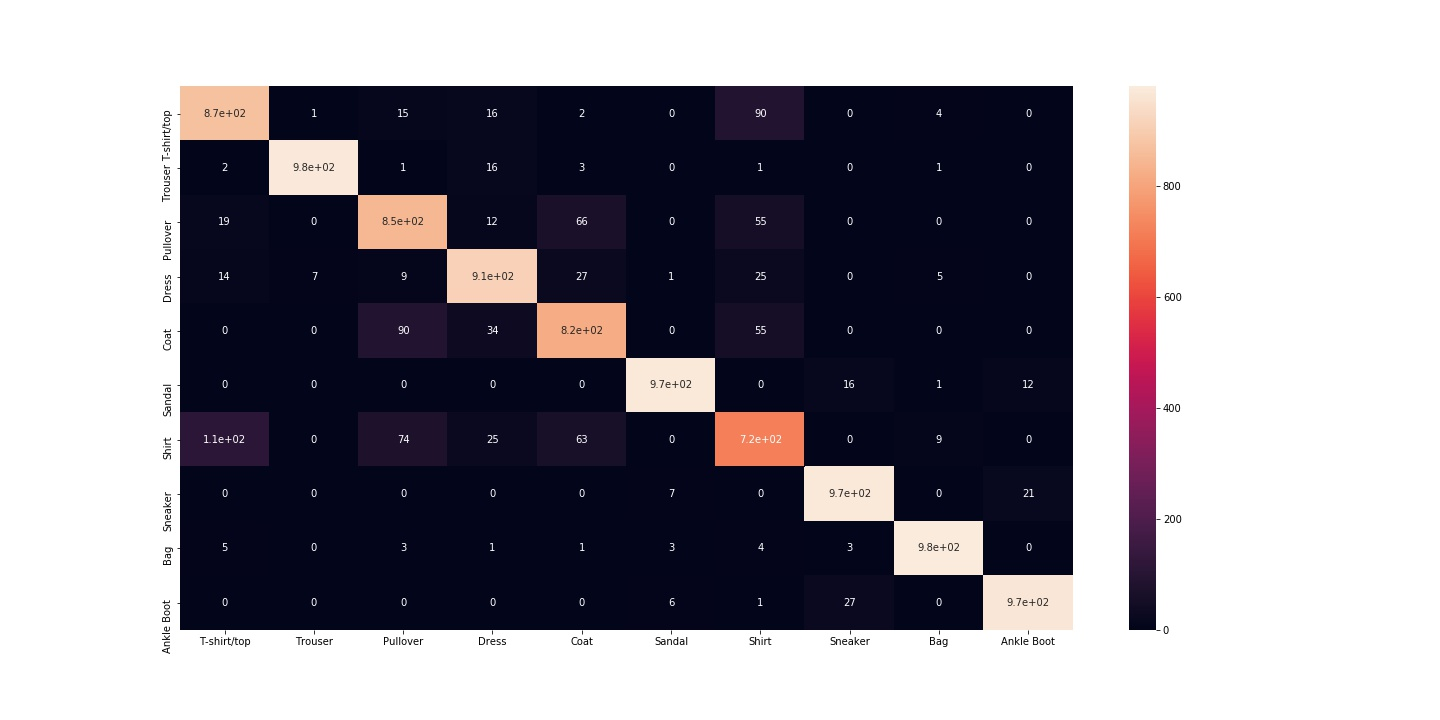
\includegraphics[width=1.3\linewidth]{cm_mlp.jpg}
	\caption{MLP Confusion Matrix}
	\label{mlpcm}
%\end{center}
\end{figure}

\subsection{Convolution Neural Network (CNN)}

Next we'll experiment with CNNs and will follow the same approach as MLP i.e. We'll start with simple baseline model and gradually improve it.

Starting with simple model with 1 convolutional layer with 1 fully connected layer. Convolutional layer will have 5x5 kernel with a stride of 1 and padding of 2. We'll use 32 filters. Since output is one of the 10 classes, throughout experiments output layer would have 10 units. It's a multi-class classification problem thus I'll be using CrossEntropy loss. ReLu is good default choice for activation function to begin experiment, we'll see how other activation functions compare. I have used Adam optimizer with 1e-3 learning rate, which will be tuned during hyper parameter tuning phase.

	This simple baseline model gives accuracy of 91.03\% on the validation set. Figure \ref{mlploss} shows the training loss decreasing with no of epocs. Training is stopped at 30 epocs since further training gives no performance gain in validation set accuracy. We'll stick to 30 epocs for further experiments for fair comparison. \\

\begin{figure}[h!]
\begin{center}
	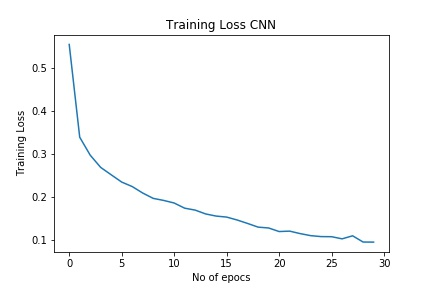
\includegraphics[width=0.85\linewidth]{training_cnn.jpg}
	\caption{CNN Loss}
	\label{mlploss}
\end{center}
\end{figure}

\pagebreak

	Next we'll increase the capacity of network by adding additional layers. Figure \ref{mlpval} shows the performance of the network with additional layers. Slight drop in accuracy suggest the possibility of over-fitting in network. We'll keep the no of convolutional layers to 4 where the over-fitting has just started and explore regularization methods to further increase accuracy.

\begin{figure}[h!]
\begin{center}
	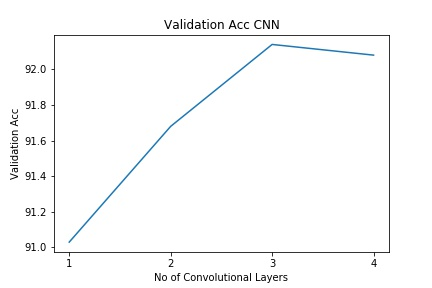
\includegraphics[width=0.85\linewidth]{val_cnn.jpg}
	\caption{CNN Val Acc}
	\label{mlpval}
\end{center}
\end{figure}
	
\textbf{Regularization:} Following forms of regularization were tried, it was also observed that combining multiple forms of regularization does improve performance.\\

\begin{enumerate}
\item \textbf{Normalization} We'll use normalize transform on the dataset to get 0 mean and unit variance. Additionally we'll apply \textbf{BatchNorm} after every conv layer and fully connected layer. BatchNorm has been shown to be very useful in CNNs and here we did see performance gain due to it. Resultant model gives 92.25\% validation accuracy. 

\item \textbf{L2 penalty} L2 regularization is another widely used regularization method for linear models. It's rarely used in DNN computer vision tasks, here the resultant model gives 89.66\% accuracy.

\item \textbf{Dropout} It's the de-facto regularization method for computer vision tasks and shown to prevent over-fitting in wide variety of network architectures. Here the resultant model gives 92.94\% accuracy.

\item \textbf{Data Augmentation} It is often used when dealing with smaller datasets where we augment the dataset to increase the size, it helps in reducing over-fitting. We'll use RandomHorizontalFlip for data augmentation. Here the resultant model gives 92.42\% accuracy. Adding random noise for data augmentation shows no improvement but further reduces accuracy.

\end{enumerate}

Using normalization, dropout and data augmentation together gives the best results and we the resultant accuracy turns out to be 93.57\%.

Next we try different activation functions i.e. Sigmoid, Tanh, ReLU. as expected ReLU performs the best from the alternatives. Sigmoid and Tanh gives 0.43\% and 0.90\% reduction in accuracy respectively when compared against ReLU.

\textbf{Hyper-Parameters tuning} After choosing the best model so far i.e. model with 4 convolutional layers and dropout regularization along with normalization and data augmentation with ReLU activation function, we'll tune the remaining hyper-parameters.
\begin{enumerate}
\item \textbf{Learning rate} is probably the most important hyper parameter, I've started with good default of 1e-3 and used "ReduceLROnPlateau" learning rate scheduler in PyTorch. It gradually decreases the learning rate upon reaching a plateau. Here for the scheduler to work better, the model is trained for 60 epocs. Resultant model gives accuracy of 94.23\% on validation set.

\item \textbf{Batch Size} affects both the training speed and the accuracy of resultant model, I have tried several values for batch size and 512 gives the best results.

\end{enumerate}

After all hyper-parameter tuning and using learning rate scheduler (training upto 60 epocs) we get a validation accuracy of \textbf{94.23\%.}. Table \ref{table:2} gives the summary of overall experiments.

\begin{table}[h!]
\centering
\begin{tabular}{|c| c|} 
 \hline
 Model & Validation Accuracy (\%) \\
 \hline\hline
 Baseline (1 conv layer) & 91.03 \\ 
 \hline
 4 conv layers with BatchNorm & 92.25 \\ 
 \hline
4 conv layers with L2 penalty & 89.66 \\ 
 \hline
 4 conv layers with dropout & 92.94 \\ 
 \hline
4 conv layers with data aug & 92.42 \\ 
 \hline
4 conv layers with norm, dropout and aug & 93.57 \\ 
 \hline
4 conv layers with norm, dropout and aug and HP tuning & \textbf{94.23} \\ 
 \hline

\end{tabular}
\caption{Summary of different architectural choices (CNN) }
\label{table:2}
\end{table}

Finally we take the best performing model and test the performance on actual test set. Here it gives \textbf{accuracy of 93.68\%}. Figure \ref{cnncm} shows the confusion matrix for test data. As expected most of confusion lies between classes such as Shirt vs Tshirt, Coat vs Pullover and Shirt vs Pullover which is justified given the visual similarity between the classes. This suggests that model has captured the differences between classes to a good extent.

\begin{figure}[h!]
%\begin{center}
	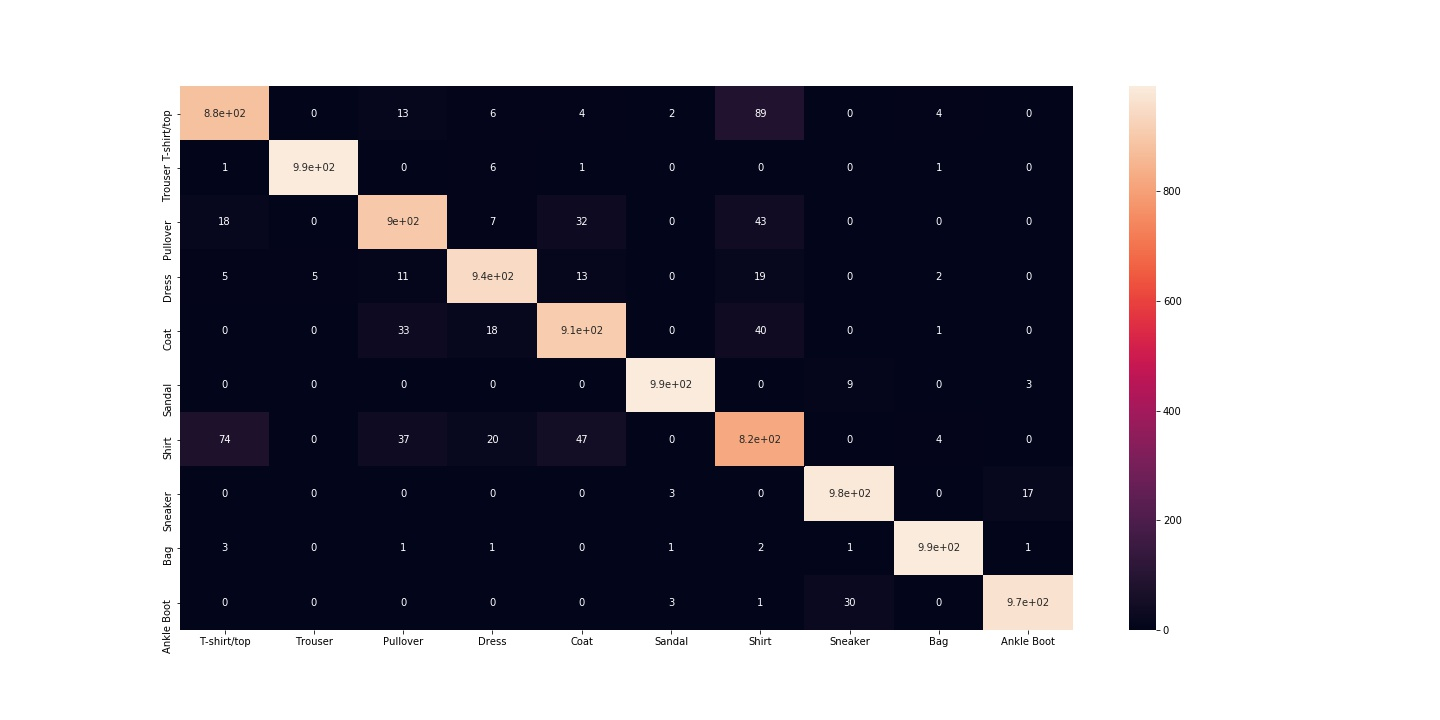
\includegraphics[width=1.3\linewidth]{cm_cnn.jpg}
	\caption{CNN Confusion Matrix}
	\label{cnncm}
%\end{center}
\end{figure}

Table \ref{table:3} shows the performance of both MLP and CNN on the actual test dataset. CNN clearly performs better than MLP with \textbf{3.34\%} better accuracy.

\begin{table}[h!]
\centering
\begin{tabular}{|c| c|} 
 \hline
 Model & Test Set Accuracy (\%) \\
 \hline\hline
MLP & 90.34 \\ 
 \hline
CNN & 93.68 \\ 
 \hline

\end{tabular}
\caption{Result on test dataset }
\label{table:3}
\end{table}


\bibliographystyle{IEEEtran}
\bibliography{references.bib}
\end{document}
